\section{Reverse Proxy}

Um servidor \textit{Reverse Proxy} transfere os pedidos dos clientes para esses servidores. Os \textit{Reverse Proxy} são geralmente utilizados para aumentar a proteção, a velocidade e a fiabilidade. Um \textit{Reverse Proxy} recebe o pedido de um cliente, passa-o para outro servidor, e depois reencaminha-o de volta para o cliente, fazendo-o parecer como se fosse o servidor proxy inicial. \textit{Reverse Proxy} asseguram que os utilizadores não chegam diretamente ao servidor de origem, fornecendo assim anonimato a este servidor web.

\textit{Reverse Proxy} podem proteger os servidores web, aumentar o desempenho do website, e ajudar a evitar a sobrecarga. Os \textit{Reverse Proxy} são também utilizados para balanceamento de carga, caching, e encriptação \ac{SSL}.

\begin{figure}[H]
\center
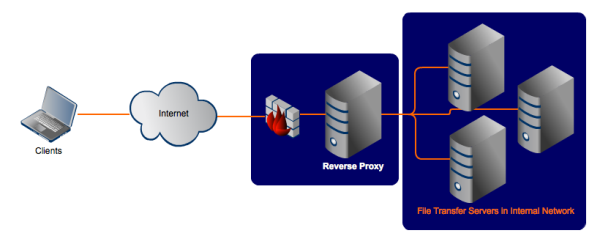
\includegraphics[width=12cm]{reverse_proxy.png}
\caption{Reverse Proxy}
\end{figure}

\section{Forward Proxy}

\textit{Forward Proxy} atua como intermediário entre os utilizadores e os servidores web. Isto significa que o pedido do utilizador passa primeiro pelo \textit{Forward Proxy} e depois chega à página web. Estes são enviados para o servidor proxy, redirecionando-os de volta para o utilizador. O pedido é feito pelo próprio servidor proxy e não pelo utilizador.
Uma vez que um \textit{Forward Proxy} pode ser visto como um ponto de acesso e controlo, pode aumentar a segurança dos utilizadores dentro de uma rede privada.

\begin{figure}[H]
\center
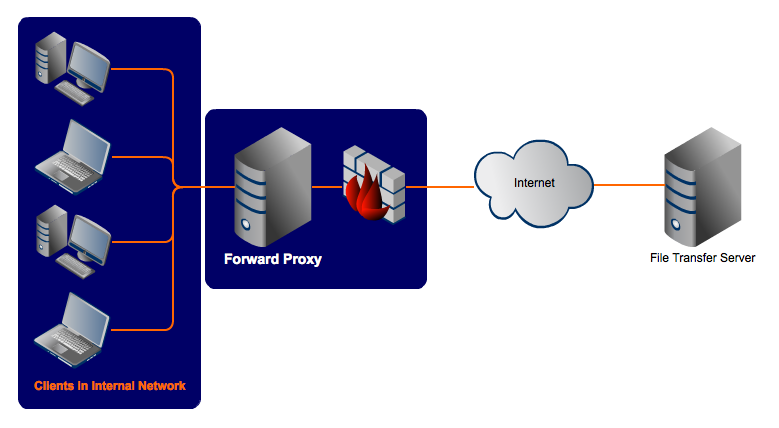
\includegraphics[width=12cm]{forward_proxy.png}
\caption{Forward Proxy}
\end{figure}